\documentclass[12pt,letterpaper]{article}
\usepackage{amsmath,amsthm,amsfonts,amssymb,amscd}
\usepackage{listings}
\usepackage{color}

\definecolor{dkgreen}{rgb}{0,0.6,0}
\definecolor{gray}{rgb}{0.5,0.5,0.5}
\definecolor{mauve}{rgb}{0.58,0,0.82}

\lstset{%frame=tb,
  language=Bash,
  aboveskip=3mm,
  belowskip=3mm,
  showstringspaces=false,
  columns=flexible,
  basicstyle={\small\ttfamily},
  numbers=none,
  numberstyle=\tiny\color{gray},
  keywordstyle=\color{blue},
  commentstyle=\color{dkgreen},
  stringstyle=\color{mauve},
  breaklines=true,
  breakatwhitespace=true
  tabsize=3
}


\usepackage{hyperref}
\usepackage{graphicx}
\usepackage{enumerate}
\usepackage{fancyhdr}
\usepackage{mathrsfs}
\usepackage[margin=3cm]{geometry}
\setlength{\parindent}{0.0in}
\setlength{\parskip}{0.05in}

% Edit these as appropriate
\newcommand\course{CS595}
\newcommand\semester{FAll 2013}     
\newcommand\hwnum{6}
\newcommand\yourname{Amara Naas}
\newcommand\login{anaas}
\newcommand\DATE{10/31/2013}

\newenvironment{answer}[1]{
  \subsubsection*{Problem #1}
}

\pagestyle{fancyplain}
\headheight 40pt
\lhead{\yourname\ (\login)\\\course\ --- \semester}
\chead{\textbf{\Large Assignment \hwnum}}
\rhead{\DATE}
\headsep 40pt

\begin{document}

\begin{answer}{1}
In this assignment I used igraph in R to find out the answer for this question. In the file called {\it ScriptR.r}\footnote{File uploaded to github} 

\begin{itemize}
\item I imported the data from \url {http://igraph.sourceforge.net/karate.net} and assigned it to "g" and plotted the graph as shown in (Figure 1) which representing the result of Zachary's paper \footnote{Zachary, 1977, http://aris.ss.uci.edu/~lin/76.pdf}.
 

\item Loop on the data and find the maximum edge betweenness value by using:\linebreak
 \textcolor{red}{[max(edge.betweenness(g))]}.
\item Find the index of the edge that has the maximum edge betweenness value and delete it from the graph  by using \textcolor{red}{[delete.edges(g, E(g,get.edge(g,i)))]}.
\item When I get two clusters the while loop stops and the graph is plotted as shown in (Figure 2). 
\end{itemize}

The results that I got from (Figure 2) is very close to the result's of the paper\footnotemark[1] where only node 3 was moved from first cluster in the paper to the second cluster in the paper.  


\end{answer}

\begin{figure}
	\center
		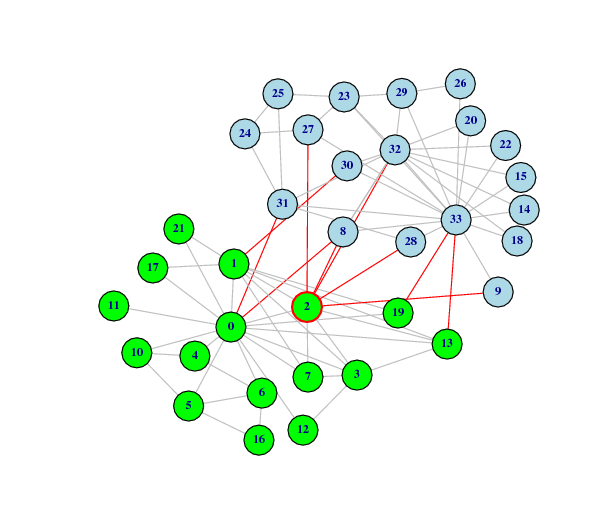
\includegraphics[width=\linewidth]{Scriptr.png} 
	\caption{Community Before Splitting}
\end{figure}
\begin{figure}
	\center
		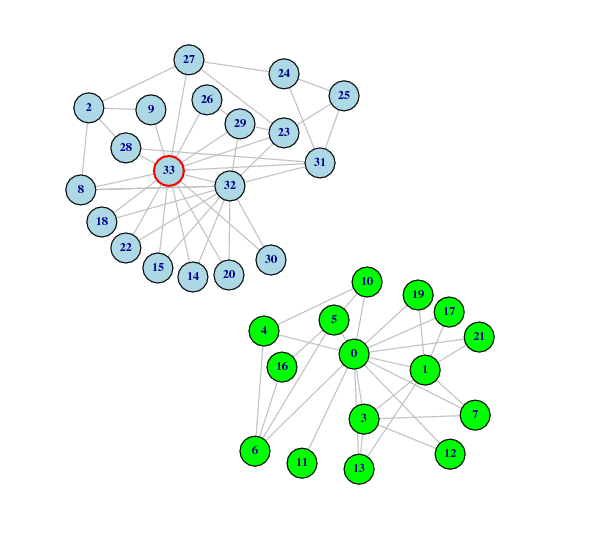
\includegraphics[width=\linewidth]{Scriptr2.png} 
	\caption{Community After Splitting}
\end{figure}

\end{document}